\chapter{OpenBTS}

\section{What is OpenBTS?}
OpenBTS is a Unix application that uses a software radio to present a GSM Um interface to handsets and uses a SIP softswitch or PBX to connect calls.(You might even say that OpenBTS is a simplified form of IMS that works with 2G feature-phone handsets). The combination of the global -standard GSM air interface with low cost VoIP backhaul forms the basis of a new type of cellular network that can be deployed and operated at substantially lower cost than existing technologies in many applications, especially rural cellular deployments and private cellular networks in remote areas.

\section{The OpenBTS Application Suite}
A complete OpenBTS P2.8 installation comprises several distinct applications:

\begin{description}
\item[OpenBTS] The actual OpenBTS application, containing most of the GSM stack above the radio modem.
\item[Transceiver] The software radio modem and hardware control interface.
\item[Asterisk] The VoIP PBX in the standard public release configuration.
\item[Smqueue] The store-and-forward server for text messaging.
\item[Subscriber Registry] A database of subscriber information that replaces both the Asterisk SIP registry and the GSM Home Location Register (HLR).
\item[Other Servers] Other optional GSM services, beyond speech and text messaging, are supported through external servers.
\end{description}

The OpenBTS and Transceiver applications must run inside each GSM/SIP access point. The Asterisk and the subscriber registry applications are communicated through the filesystem and therefore must run on the same computer, but that computer can be remote from the access point. smqueue and the other servers can run anywhere and may have multiple instances.

 \subsection{OpenBTS}
The OpenBTS application contains:
\begin{itemize}
\item L1 Time division multiplexing(TDM) functions (GSM 05.02)
\item L1 Forward error correction(FEC) functions (GSM 05.03)
\item L1 closed loop power and timing controls (GSM 05.08 and 05.10)
\item L2 Link access protocol on Dm-channel (LAPDm) (GSM 04.06)
\item L3 radio resource management functions (GSM 04.08)
\item L3 GSM-SIP gateway for mobility management
\item L3 GSM-SIP gateway for call control
\item L4 GSM-SIP gateway for text messaging
\end{itemize}

The general design approach of OpenBTS is avoid implementing any function above L3, so at L3 or L4 every subprotocol of GSM is either terminated locally or translated through a gateway to some other protocol for handling by an external application. Similarly, OpenBTS itself does not contain any speech transcoding functions above the L1 FEC parts.

\subsection{Transceiver}
The transceiver application performs the radio modem functions of GSM 05.05 and manages the Gigabit Ethernet interface
(USB2 interface, in case
of USRP1 or older models) to the radio hardware.

\subsection{Asterisk}
OpenBTS uses a SIP switch or PBX to perform the call control functions that would normally be performed by the mobile switching center in a conventional GSM network, although in most network configurations this switching function is distributed over multiple switches. These switches also provide transcoding services. In OpenBTS P2.8 the standard SIP switch is Asterisk 1.8.

\subsection{Subscriber Registry}
OpenBTS uses a modified SIP registry as a substitute for the home location register found in a conventional GSM network. OpenBTS also relies on Asterisk for any transcoding functions.

\subsection{Smqueue}
Smqueue is a store-and-forward server that is used for text messaging in the OpenBTS system. Smqueue is required to send a text message from one MS to another, or to provide reliable delivery of text messages to an MS from any source.

\subsection{Network Organization}
In the simplest network, with a single access point, all of the applications
in the suite run inside the access point on the same embedded computer. Figure
\ref{btsSimple} describes this.



\begin{figure}
\centering
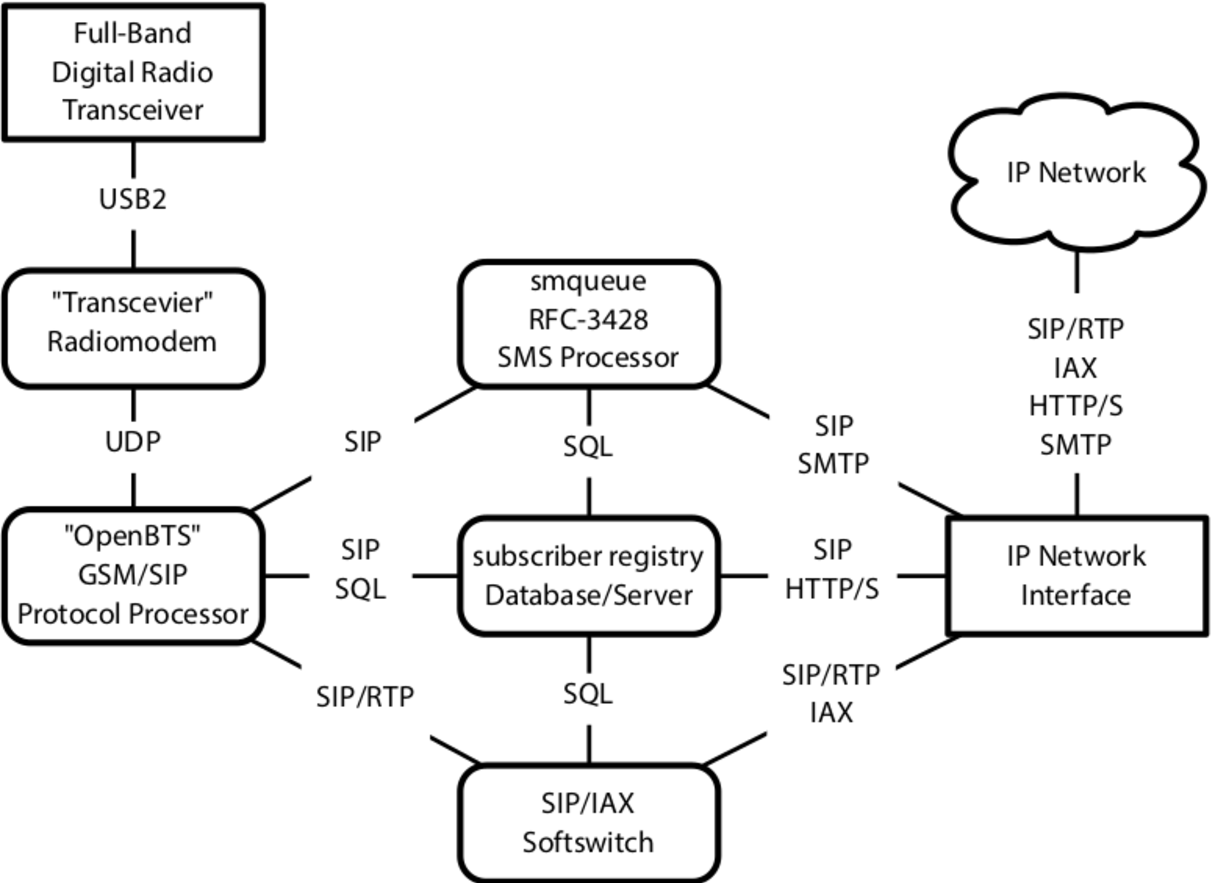
\includegraphics[width=1\textwidth]{../images/btsSimple}
\caption[Network Organization of OpenBTS]{\textbf{Network Organization of OpenBTS}: The smqueue block handles SMSs.
The subscriber registry database contains the details of all registered users and it
maps the registered IMSIs to corresponding dialling numbers. The softswitch connects
speech calls (e.g. Asterisk, FreeSwitch). The transceiver performs radio modem
functions and manages the Gigabit Ethernet interface (USB2 interface, in case
of USRP1 or older models) to the USRP device. The OpenBTS itself is the GSM
implementation from the TDMA part of L1 up through L3 and the L3/L4 boundary.
It has a SIP interface to communicate with the other blocks like smqueue, subscriber
registry, etc {\cite{openbtsMan}}.}
\label{btsSimple}
\end{figure}

In larger network, with more than one access points, one of the BTS can behave as a master
and provide servers to the rest of them. Figure \ref{fig:btsLarge} describes a network with two access points
where a master access points is providing servers to the other one.
The Transceiver applications and the OpenBTS must run in each GSM/SIP access point.
The Asterisk and the Subscriber Registry applications (SIPAuthServe) communicate via the
filesystem and hence must run in the same computer, but that computer can be remote to the
access point. SMQueue and other servers can run in any access point and can have multiple
instances.
\begin{figure}
  \centering
    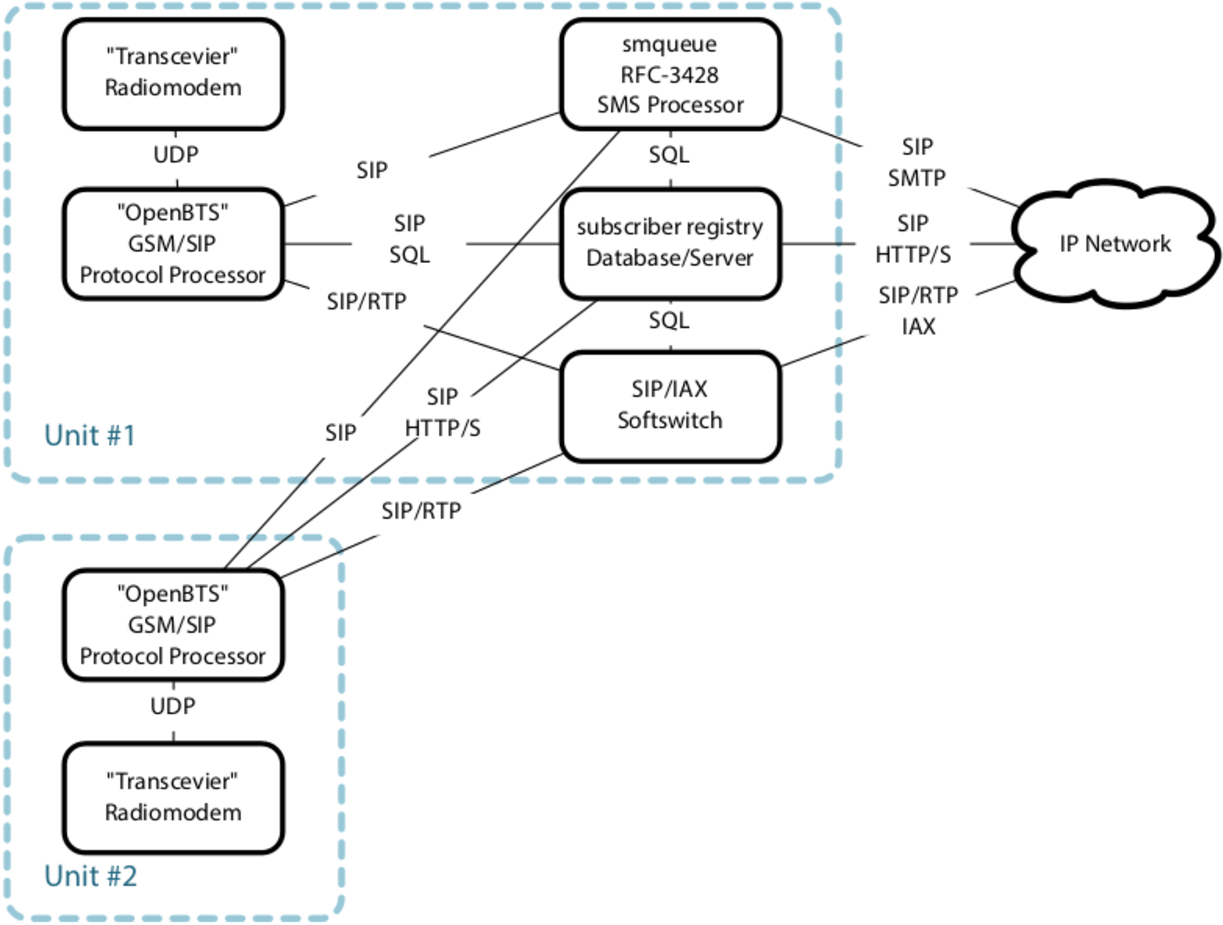
\includegraphics[width=\textwidth]{../images/btsLarge}
  \caption[OpenBTS network with two access points]{Two access points with unit 
  \#1 providing servers for both {\cite{openbtsMan}}.}
  \label{fig:btsLarge}
\end{figure}






